\section{Driving a race car}
\label{sec:driving_race_car}
In order to allow the two models to drive a race car in the Car Racing environment, they should be included in a feedback loop, as shown in Figure \ref{fig:game_loop}. Based on an initial observation, the agent (the CNN) takes an action, which is passed to the environment. The environment then computes a response and returns a new observation, which is passed to the agent. The agent then takes another action, and so on, until the game ends (because of the car either crashing or completing a full lap, or because of the expiration of the maximum time of 30 seconds).

\tikzstyle{block} = [rectangle, draw, fill=gray!20, align=center, rounded corners, minimum height=1cm, font=\small]

\begin{figure}[htbp]
    \centering
    \begin{tikzpicture}
        \node [block] (block1) {Agent (CNN)};
        \node [block, right=2cm of block1] (block2) {Environment};
        
        \path[->] (block1) edge [bend left=45] node[above] {Action} (block2);
        \path[->] (block2) edge [bend left=45] node[below] {Observation} (block1);
    \end{tikzpicture}
    \caption{Closed loop between the CNN and the Car Racing environment.}
    \label{fig:game_loop}
\end{figure}


\noindent Mainly due to the class weights choice of Sec. \ref{sec:effect_of_class_weights}, both the models are capable of playing the racing game with a good degree of success on a great number of randomly-generated tracks, as shown in Fig. \ref{fig:car_racing} and in the video linked in the footnote\footnote{YouTube video showing the two models driving on randomly-generated tracks: \url{https://youtu.be/EUGlU5wEMvg}}. However, there is still a lot of room for improvement, as the models sometimes act in a way that is not optimal and that can possibly lead to "crashes", as shown in Fig. \ref{fig:car_racing_fail}. With this in mind, it would probably be best to combine a CNN model with one of reinforcement learning that also exploits the reward system of the Gym environment.

\begin{figure}[htbp]
    \centering
    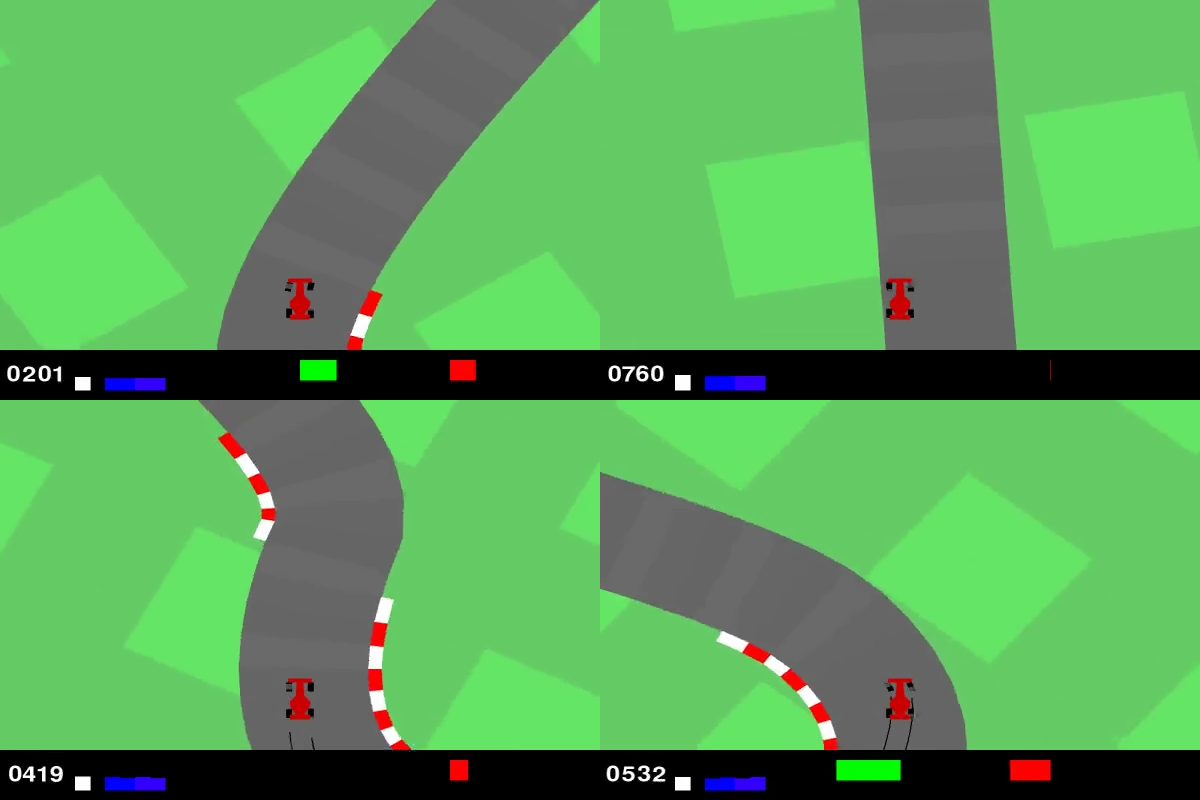
\includegraphics[width=0.75\textwidth]{figures/images/car.png}
    \caption{The models driving in the Car Racing environment.}
    \label{fig:car_racing}
\end{figure}


\begin{figure}[htbp]
    \centering
    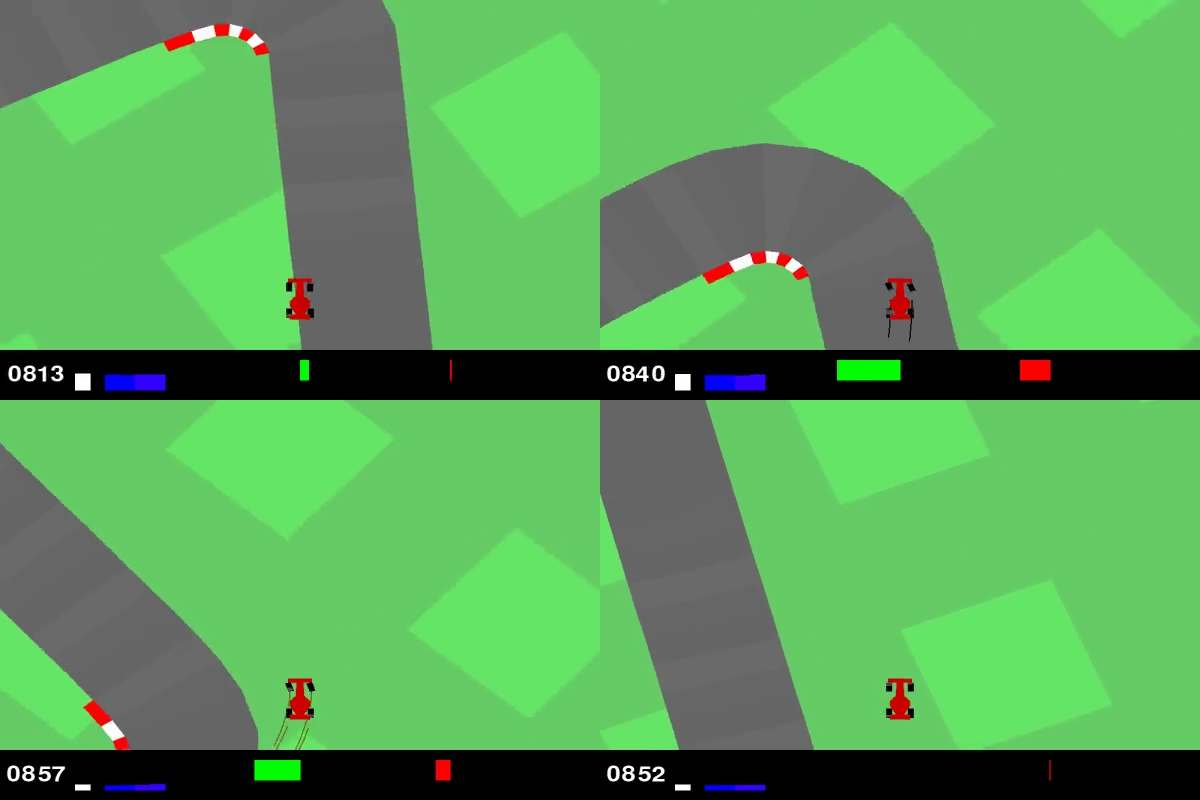
\includegraphics[width=0.75\textwidth]{figures/images/car_fail.png}
    \caption{Model 0 causing the race car to skid off the road.}
    \label{fig:car_racing_fail}
\end{figure}



